\documentclass[../main]{subfiles}
\ifSubfilesClassLoaded{
    \addbibresource{../Biblio/biblio.bib}
    \dominitoc
    \tableofcontentsfile
    \pagenumbering{arabic}
    \setcounter{page}{1}
}{}
\begin{document}
\chapter{Information mutuelle normalisée comme indicateur de l'apprentissage des données multimodales\label{chap:indicateur}}
\graphicspath{{05-Indicateur/},{./figures/}}
\minitoc

Dans le chapitre précédent, nous avons présenté différents tracés permettant de conclure que l'architecture de cartes extrait une représentation interne du modèle d'entrée lors de l'apprentissage.
Cet apprentissage du modèle se caractérise par le fait que chaque carte dissocie les BMUs en fonction du modèle d'entrées global et non seulement de son entrée externe. 
La variable cachée $U$, représentant le modèle d'entrées, est alors une fonction du BMU $\bmu$ dans chacune des cartes de l'architecture, comme rappelé sur la figure~\ref{fig:upi_chap4}.
Nous souhaitons définir un indicateur numérique caractérisant cette propriété, c'est-à-dire caractérisant que $U$ est fonction de $\bmu$ dans chaque carte. Cet indicateur nous permettra  de comparer plusieurs expériences entre elles de façon numérique.
Les tracés sont réalisables pour une variable cachée $U$ en en une dimension~; un indicateur numérique nous permettra aussi d'évaluer l'apprentissage lorsque la dimension de $U$ est plus grande.

Nous avons défini les expériences en termes de variables aléatoires. La théorie de l'information de Shannon \cite{Shannon1948AMT} apporte un modèle mathématique qui permet de manipuler et encoder ces variables et quantifier l'information partagée entre leurs distributions.
Nous définirons dans ce chapitre des indicateurs permettant d'évaluer l'apprentissage du modèle par l'architecture de cartes.

\begin{figure}
    \centering
    \includegraphics[width=0.7\textwidth]{xu_yu_both_chap4.pdf}
    \caption{Rappel~: comparaison de $U$ en fonction de $\bmu\m{1}$ dans l'expérience exemple à deux cartes, sur des entrées sous forme de cercle. Ce nuage de point fait apparaître une relation semblant bijective entre $U$ et $\bmu\m{1}$. Nous définiront un indicateur permettant de représenter numériquement cette propriété.
    \label{fig:upi_chap4}}
\end{figure}

\subsection{Indicateurs envisagés}

Plusieurs méthodes permettent d'évaluer une relation statistique existant entre deux signaux. Citons notamment la corrélation croisée, le ratio de corrélation et l'information mutuelle.
La corrélation croisée cherche une ressemblance entre deux signaux de façon linéaire. Une bonne corrélation croisée traduit ainsi l'existence d'une relation linéaire entre deux signaux.
Le ratio de correlation est un rapport mesurant l'existence d'une relation fonctionnelle non-linéaire entre les deux variable. 
Enfin, l'information mutuelle permet d'évaluer une relation statistique quelconque entre les variables.

\begin{itemize}
    \item Avantages du correlation ratio: mesure précisément une relation fonctionnelle quelconque, est à valeur dans 0,1. Désavantages: besoin de passer par l'estimation des densités de proba, en particulier $U|\bmu$, donc peu pratique quand la dimension augmente.
    \item Information mutuelle : mesure une relation statistique quelconque. Largement utilisé, donc de nombreuses méthodes fiables d'estimation existent, y compris pour des dimensions supérieures. Normalisation possible pour définir un indicateur compris entre 0 et 1. Est maximale lorsque qu'il existe une bijection entre les deux variables, ce qui est ce qu'on veut mesurer.
\end{itemize}

\section{Rappel des éléments de théorie de l'information}

Les notions d'\emph{entropie} et les valeurs associées, telle que l'\emph{information mutuelle} entre des distributions, sont des notions fondamentales de la théorie de l'information de Shannon. Ces quantités sont liées à la distribution d'une variable aléatoire.
L'entropie de Shannon d'une variable aléatoire $X$ à valeurs discrètes dans un ensemble $E_X$, de distribution $P_X$, est notée $H(X)$ et définie par la formule : 
\begin{equation}
H(X) = - \sum_{x \in E_X}{P_X(x)\textrm{log}(P_X(x))}
\end{equation}

Elle se mesure en $bit/symbole$ lorsque le logarithme est en base 2, ce qui est généralement utilisé. 
L'entropie est une mesure de la quantité d'incertitude, ou de surprise, sur la valeur de la variable aléatoire $X$. Si la la distribution de probabilité de $X$ est concentrée autour d'un point, l'entropie est faible : lors d'une réalisation de $X$, l'observateur est \emph{plutôt certain} du résultat. En revanche, l'entropie est maximale lorsque lorsque $X$ suit une distribution de probabilité uniforme.
L'entropie s'interpète également comme la quantité moyenne d'information à fournir, en bits, pour coder la valeur que prend la variable $X$.
De la même manière, on peut définir l'entropie conjointe de deux variables, qui est l'entropie de leur distribution jointe, et l'entropie conditionnelle, qui est l'entropie de leurs distributions conditionnelles.

Outre les entropies jointes et conditionnelles, l'existence d'une relation statistique entre deux variables aléatoires $X,Y$ à valeurs dans $E_X,E_Y$ se mesure par \emph{l'information mutuelle}. Elle se définit formellement par : 
\begin{equation}
 I(X,Y) = \sum_{x,y \in E_X,E_Y}{P_{XY}(x,y)\textrm{log}(\frac{P_{XY}(x,y)}{P_X(x)P_Y(y)})}
\end{equation}
Cette valeur mesure la quantité d'information moyenne partagée entre les distributions $X$ et $Y$: en moyenne, quelle information sur la valeur de $Y$ donne une valeur de $X$ et inversement, quelle information sur la valeur de $X$ donne une valeur de $Y$.

L'information mutuelle possède les propriétés suivantes:
\begin{enumerate}
\item $I(X,Y) = 0 \Leftrightarrow \textrm{X et Y sont indépendantes}$. L'information mutuelle peut être vue une mesure de la distance entre la distribution jointe de $(X,Y)$, $P(X,Y)$ et la distribution dans laquelle les deux variables sont indépendantes, $P(X)P(Y)$.
\item Elle s'exprime à partir de l'entropie : $I(X,Y) = H(X) + H(Y) - H(X,Y) = H(X) - H(X|Y) = H(Y) - H(Y|X)$
\item Elle est symétrique : $I(X,Y) = I(Y,X)$
\item Pour toute fonction $f$, $I(X,Y) \geq I(X,f(Y))$. L'égalité est atteinte si et seulement si $f$ est \emph{bijective}.
\end{enumerate}

Lors de l'analyse de CxSOM, on s'interroge sur l'information que portent les positions des BMUs $\bmu$ d'une carte sur le modèle d'entrée.
Les éléments de la carte ont été définis en termes statistiques~; on peut donc utiliser l'information mutuelle comme une représentation de l'information partagée entre la position du BMU d'une carte et la variable paramétrant le modèle d'entrée, $U$.


\section{Utilisation du ratio de corrélation comme mode d'évaluation}

Nous cherchons à mesurer la dépendance fonctionnelle existant entre la variable $\bmu\m{i}$, les positions du BMU d'une carte, et la variable $U$ décrivant le modèle.
Le ratio de corrélation $\eta(\bmu\m{i},U)$ permet de mesurer un coefficient de dépendance non-linéaire entre deux variables, ce qui correspond à une relation fonctionnelle. Il atteint la valeur de 1 lorsque $U$ est fonction de la première variable $\bmu\m{i}$ et est nul lorsque les deux variables sont statistiquement indépendantes.
A ne pas confondre avec le coefficient de Pearsons $r$ qui mesure une dépendance linéaire. Cependant, eta rejoint r lorsque (??)


\subsection{Définition}

La mesure de la dépendance fonctionnelle entre deux variables $X$ et $Y$ peut se décomposer en deux étapes:
\begin{enumerate}
    \item Trouver une fonction $\varphi(X)$ qui approxime les valeurs de $Y$
    \item Mesurer la qualité de l'approximation.
\end{enumerate}

La fonction $\varphi$ considérée pour le calcul du ratio de corrélation est ici~:
\begin{equation}
    \varphi = \mathbb{E}(Y|X)
\end{equation}

Il s'agit bien d'une fonction de $X$. Un exemple de calcul de $\varphi$ est illustré en figure~\ref{fig:cr_box}, estimé par discrétisation des valeurs de $X$. Il s'agit en fait de la fonction approximant au mieux les valeurs de $Y$.

Le ratio de corrélation $\eta$ mesure ensuite la qualité de l'approximation des valeurs de $Y$ par la fonction $\varphi$ en faisant le rapport des variances de ces deux variables~:
\begin{equation}
    \eta(Y|X) = \frac{Var(\mathbb{E}(Y|X))}{Var(Y)}
\end{equation}

On peut mieux comprendre la signification de ce coefficient en modifiant un peu l'équation.
Par la définition des variances conditionnelles, on a 
$$Var(Y) = \mathbb{E}(Var(Y|X)) + Var(\mathbb{E}(Y|X))$$
Soit~:
$$\eta(Y|X) = 1 - \frac{\mathbb{E}(Var(Y|X))}{Var(Y)}$$
$\mathbb{E}(Var(Y|X))$ représente la moyenne des écarts de $Y|X=x_i$ à sa valeur moyenne en $x_i$ $\mathbb{E}(Y|X=x_i)$ pour une valeur de $X = x_i$ donnée. Lorsque la dépendance entre $Y$ et $X$ est fonctionnelle, les valeurs de $Y|X$ sont très proches de $\mathbb{E}(Y|X)$ pour chaque valeur de $X$ et $\mathbb{E}(Var(Y|X))$ est faible partout. La variance est nulle lorsqu'une valeur de $X$ correspond à un seul point pour $Y$, c'est à dire une relation fonctionnelle. Inversement, quand $Y$ et $X$ sont indépendantes, $\mathbb{E}(Var(Y|X)) = Var(Y)$ et le ratio de corrélation tombe ainsi à 0.
Le ratio de corrélation n'est pas symétrique. Par le fait qu'il s'appuie sur un rapport, il n'est pas sensible à une transformation linéaire de $Y$.

\begin{figure}
    \centering
    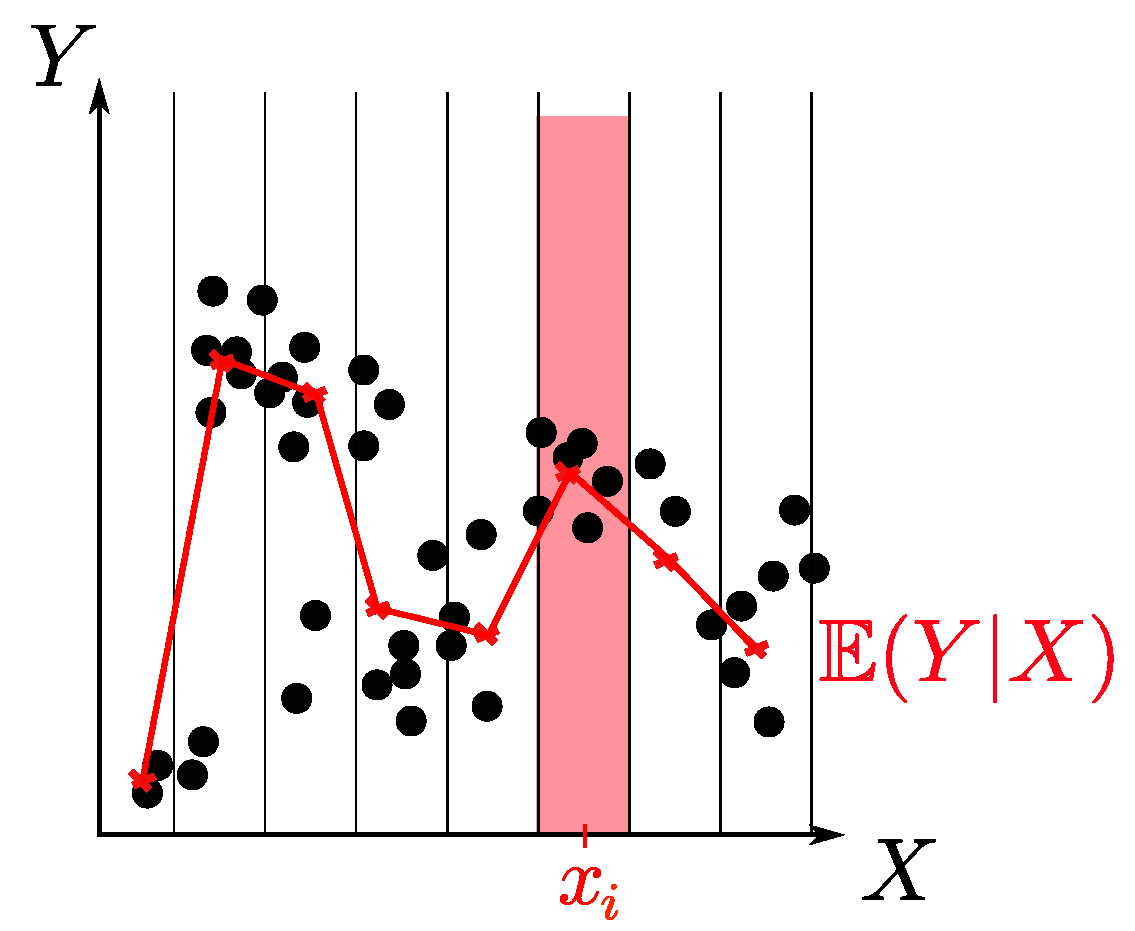
\includegraphics[width=0.6\textwidth]{boxes_CR.pdf}
    \caption{Exemple d'approximation non-linéaire de la relation entre $X$ et $Y$ par $\mathbb{E}(Y|X)$. Cette approximation est ici réalisée en discrétisant les valeurs de $X$. La valeur de la fonction pour chaque $x_i$ est alors la moyenne des valeurs de $Y$ sur l'intervalle considéré.}
\end{figure}

\subsection{\'Evolution du ratio de corrélation au cours de l'apprentissage des cartes CxSOM}

Nous utilisons le ratio de corrélation pour mesurer la dépendance fonctionnelle existant dans chaque carte entre les valeurs de $U$ et l'ensemble des BMU d'une carte $\bmu\m{i}$.
Les valeurs $\bmu\m{1}$ et $\bmu\m{2}$ étant des valeurs discrètes, $\mathbb{E}(U|\bmu\m{i})$ est estimée par la moyenne des valeurs de $U$ ayant pour BMU la même valeur $\bmu\m{i}$. 
En figure~\ref{fig:cr_xp}, nous traçons les distributions de $U$ en fonction de $\bmu\m{1}$ et $\bmu\m{2}$, dans le cas de l'architecture CxSOM et des cartes simples. Nous y représentons la fonction $\mathbb{E}(U|\bmu\m{i})$ en rouge.
Le ratio de corrélation apparaît ici comme une bonne mesure de la relation fonctionnelle existant entre $U$ et $\bmu$. Le ratio de corrélation est très proche de 1 dans chaque carte de CxSOM, traduisant le fait que $U$ est une fonction du BMU dans chaque carte.

La figure~\ref{fig:cr_bruit} présente les mêmes paramètres tracés dans le cas ou l'expérience est réalisée sur des données bruitées, en l'occurence un anneau. $U$ n'est alors plus vraiment une fonction du BMU, mais en reste proche. 
Le ratio de corrélation traduit correctement cette proximité et reste plus élevé dans chaque carte que pour une carte seule.

Enfin, nous tracons en figure~\ref{fig:cr_evol} l'évolution du ratio de corrélation sur les 200 premiers pas d'apprentissage de deux cartes sur un cercle, connectées et non connectées. Les mesures sont réalisées sur 10 expériences réalisées sur des distributions d'entrées identiques et moyennées.
Nous remarquons que $\eta$ reste inférieur dans le cas ou les cartes sont connectées que non connectées. 
Remarques:
\begin{itemize}
    \item Semble rester a peu près constant pendant tout l'apprentissage. Traduit le fait que dès le début de l'apprentissage, la relaxation différencie les BMUs en fonction des deux valeurs d'entrées, même quand les poids ne sont pas organisés.
    \item Pas d'information sur l'organisation topologique des poids ici: le coefficient ne traduit pas l'organisation de la carte.
    \item Grande variabilité de la valeur de $\eta$ entre les expériences, traduite ici par l'écart à la moyenne.
    \item On voit qu'entre la carte $M\m{1}$ et $M\m{2}$, $\eta$ prend une valeur bien différente, alors que la qualité de la relation est semblable. On peut donc difficilement utiliser $\eta$ de façon absolue, mais plutôt pour comparer des valeurs.
\end{itemize}

\begin{figure}
    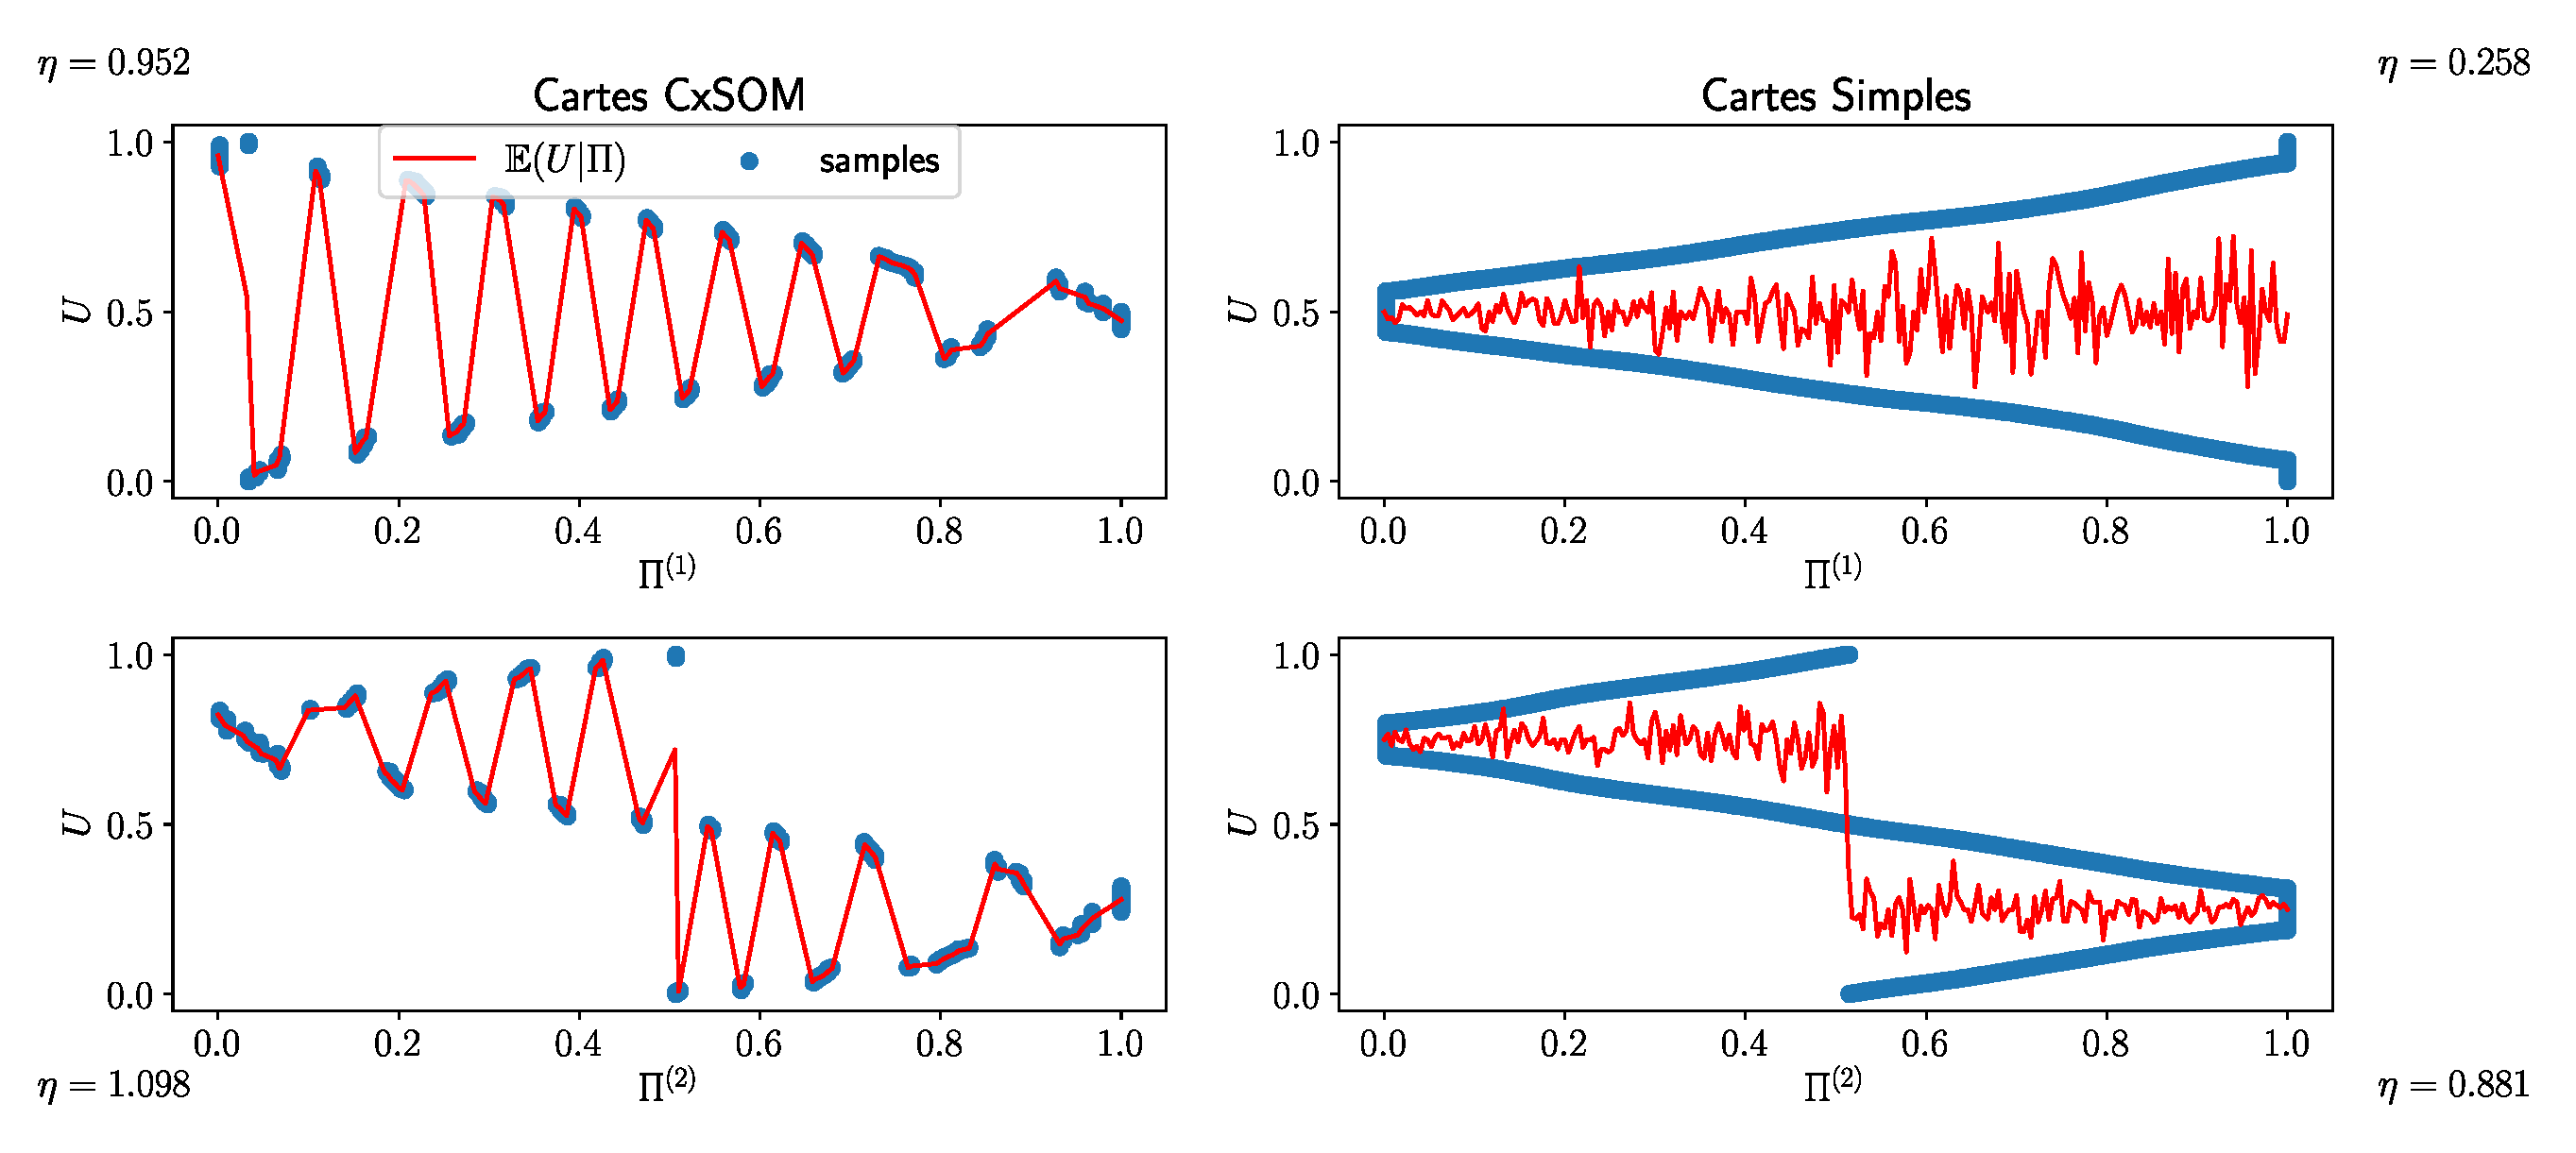
\includegraphics[width=\textwidth]{correlation_ratio_xp0.pdf}
    \caption{Tracé du ratio de corrélation sur cartes cxsom et cartes simples \label{fig:cr_xp}}
\end{figure}

\begin{figure}
    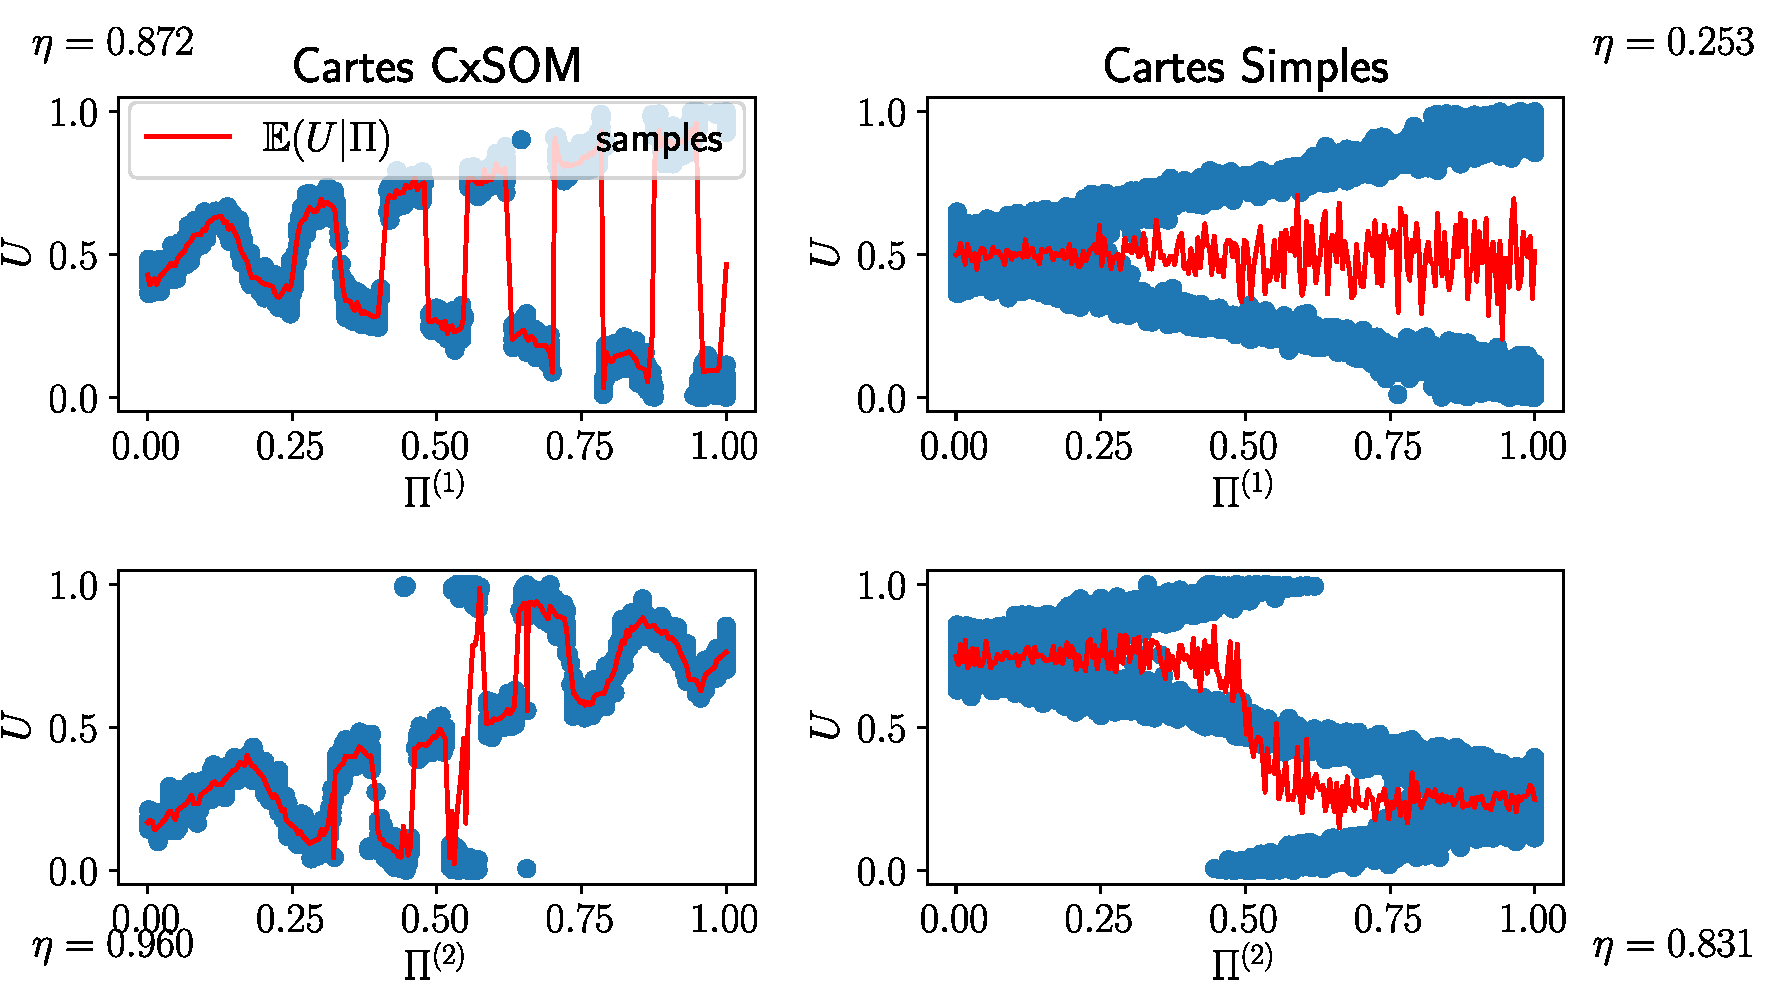
\includegraphics[width=\textwidth]{correlation_ratio_anneau_xp0.pdf}
    \caption{Tracé du ratio de corrélation sur cartes cxsom et cartes simples dans le cas ou les données sont bruitées.\label{fig:cr_bruit}}
\end{figure}

\begin{figure}
    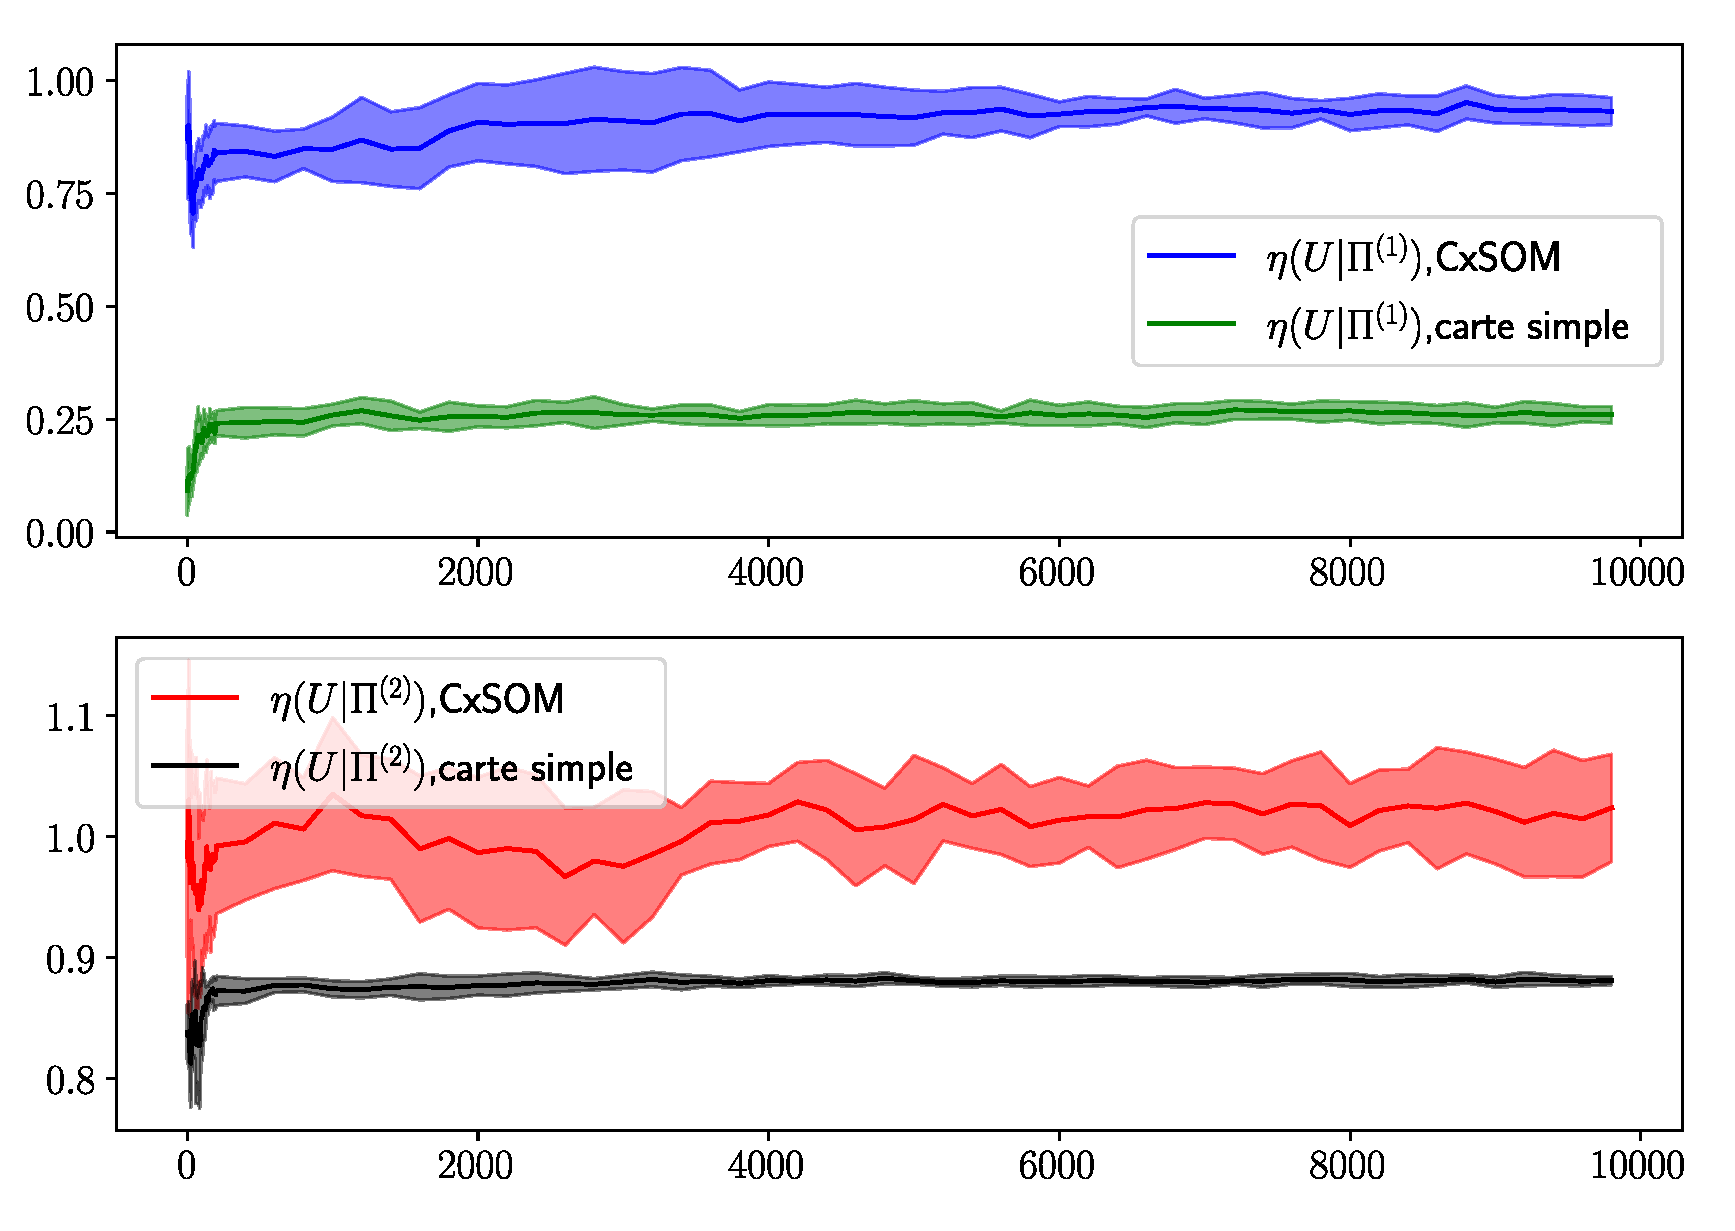
\includegraphics[width=\textwidth]{correlation_ratio_evolution_totale.pdf}
    \caption{Evolution du ratio de corrélation pendant l'apprentissage des cartes\label{fig:cr_evol}}
\end{figure}

\subsection{Discussion}
Bonne mesure de la relation existant entre $U$ et $\bmu$
Variable BMU discrète, variable U peut être continue
Très bien pour des dimensions plus grandes.

A mettre dans conclu générale: 
Néanmoins, il est montré (?) que  les variables restent sur des manifolds de dimension réduite - d'ou déjà l'intéret des cartes de kohonen et que ca marche. Donc les calculs de discretisation n'augmenteront pas de facon explosive au cours des dimensions ....


\section{Utilisation du coefficient d'incertitude comme indicateur de la relation entre $U$ et $\bmu$}

\subsection{Définition de l'indicateur}

Nous cherchons à définir un indicateur permettant d'évaluer l'apprentissage du modèle par l'architecture de cartes. D'après les observations mentionnées ci-dessus, l'existence d'un apprentissage du modèle complet se traduit par le fait que $U$ est une fonction de $\bmu$ \emph{dans chacune des cartes}.
Nous choisissons donc de définir un indicateur mesurant à quel point la variable cachée équivalente au modèle d'entrée, $U$, est une fonction de la position du BMU $\bmu$ correspondante.
Dans l'exemple, $U$ est en une dimension pour des entrées 2D $(\inpx\m{1},\inpx\m{2})$.
Nous attendons que cet indicateur prenne une valeur minimale lorsque $U$ n'a aucune relation avec $\bmu$, et augmente jusqu'à une valeur maximale lorsque $U$ est fonction de $\bmu$. Afin de pouvoir comparer les expériences entre elles, nous voulons définir un indicateur normalisé, dont la valeur est donc comprise entre $0$ et $1$.

Nous pouvons utiliser l'\emph{information mutuelle} $I(\bmu, U)$ pour évaluer l'information qu'une position du BMU d'une carte porte en moyenne sur la valeur de $U$, et $U$ sur le BMU.
L'information mutuelle dépend de la quantité d'information portée par chaque distribution et se mesure en bit/symbole. Un indicateur normalisé nous permettra de comparer des expériences différentes. 

Nous choisissons de normaliser l'information mutuelle $I(\bmu,U)$  par la valeur maximale qu'elle peut prendre dans une expérience de CxSOM. Cette valeur maximale atteinte par $I(\bmu,U)$ est $H(U)$, atteinte lorsque $U$ est une fonction de $\bmu$.
En effet, par construction, $\bmu$ est une fonction de $U$ dans une carte de Kohonen: l'algorithme est déterministe et une sortie est définie pour toute valeur de $U$. C'est à dire, $I(U,\bmu) = I (U, f(U))$.
Par propriété de l'information mutuelle, pour toute fonction $f$ et variables $X,Y$, $I(X,f(Y)) \leq I(X,Y) $. 
Donc, $I(U,\bmu) \leq I(U,U) = H(U)$
Cette valeur est atteinte si et seulement si $U$ et $\bmu$ sont en bijection, autrement dit, si et seulement si $U$ est aussi une fonction de $\bmu$.

Nous définissons donc un indicateur de la relation fonctionnelle existant entre $U$ et $\bmu$ comme:
\begin{equation}
I_x(U|\bmu) = \frac{I(\bmu,U)}{H(U)}
\end{equation}
Ce coefficient n'est pas symétrique et mesure l'information portée par le second terme sur le premier, relativement à la valeur maximale qu'il peut porter ($H(U)$). On a $I_x(U|\bmu) \in [0,1]$. Cette valeur est une variante normalisée de l'information mutuelle appelée le \emph{coefficient d'incertitude} entre $U$ et $\Pi$ et introduite par Theil en~\cite{Theil1961EconomicFA}.
Il vaut 1 lorsque $U$ est une fonction de $\bmu$ dans la carte considérée, et $0$ lorsque les deux distributions sont indépendantes. Cette relation fonctionnelle entre $U$ et $\bmu$ est bien la propriété qu'on souhaite mesurer.


%TODO : développer ce point : information portée par plus de variables !
%TODO : calculer et comparer les valeurs pour le cas du cercle.

% Ce coefficient peut être élargi à plus de variables: on peut calculer $I_x(U | (\bmu\m{1},\bmu\m{2},\bmu\m{3}))$ pour 3 cartes, en considérant la variable jointe $(\bmu\m{1},\bmu\m{2},\bmu\m{3})$.
% Plus largement, pour prouver que l'archictecture a appris un modèle, on souhaite que $I_x(U|\bmu\m{1},\cdots,\bmu\m{k})$ soit le plus proche possible de 1.
% Cet indicateur permet de comparer des expériences par des valeurs numériques, sans passer par des tracés.
\subsection{Estimation de l'indicateur}

L'information mutuelle et l'entropie sont des grandeurs définies à partir de la distribution des variables aléatoires. Ces distributions, dans notre cas, ne sont pas connues, nous devons donc estimer ces quantités à partir des échantillons de données.

\subsubsection{Méthodes d'estimation}

La méthode classique d'estimation de l'information mutuelle et de l'entropie est la méthode dite des \emph{histogrammes}.
Cette méthode s'appuie sur une estimation de la distribution des variables $U$,$\bmu$ et la distribution de la variable jointe $(U,\bmu)$ en discrétisant chacune des variables.
Cette méthode est représentée en figure~\ref{fig:binning}. Les variables $U$ et $\bmu$ sont discrétisées en \emph{boîtes} de centres $x_k$ et $y_k$ choisis.
Une distribution est alors estimée par: 
$$P(U = x_i) = \frac{n_{xi}}{N} $$ où $n_{xi}$ est le nombre d'échantillons de $U$ tombant dans la boîte de centre $x_i$ et $N$ le nombre de points. Le même procédé est réalisé pour $\bmu$ et $(U,\bmu)$. La précision de l'estimation peut être améliorée en choisissant des tailles de boîtes variables; nous utilisons ici la méthode simple avec des boites de taille fixe.
Pour des variables à valeur dans $[0,1]$, les centres sont définis par $x_k = \frac{k}{M}+\frac{1}{2M}$, avec $M$ le nombre de boîtes.
Cette discrétisation permet d'estimer les trois termes d'entropie $\hat{H}(\bmu,U)$, $\hat{H}(U)$ et $\hat{H}(\bmu)$ et d'en tirer l'information mutuelle normalisée:
\begin{equation}
    \hat{I_x}(U,\bmu) = \frac{\hat{H}(U) + \hat{H}(\bmu) - \hat{H}(U,\bmu)}{\hat{H}(U)}
   \end{equation}

La valeur de cet indicateur dépend de la résolution choisie pour l'histogramme. L'estimateur  par histogramme converge vers la valeur théorique de l'information mutuelle continue lorsque la taille des boites tend vers 0, sous réserve que les densités de probabilité existent pour chaque variable. Plus la taille des boîtes est petite, plus le nombre de points disponible pour l'estimation doit augmenter.
Notons que la méthode par histogrammes est limitée quand la dimension des entrées augmente.
Le nombre d'échantillons disponibles pour l'estimation doit augmenter exponentiellement avec la dimension des variables pour éviter le phénomène de "boîtes vides": à cause de la dispersion des données, de nombreuses boîte $(x_j,y_i)$ ne contiendront pas de points alors qu'elles auraient dû en contenir selon leur distribution; l'estimation de la distribution en ce point sera alors nulle, et l'estimation de l'indicateur faussée.

Une deuxième méthode généralement utilisée pour l'estimation de l'information mutuelle est l'estimateur par KNN (K-nearest neighbors) de Kraskov \cite{2004kraskov}. 
Cet estimateur ne passe pas par l'estimation de la densité de probabilité, contrairement aux histogrammes, mais estime directement les entropies et l'information mutuelle.
Le découpage de l'espace se fait en recherchant, pour un couple $(X,Y)$ les k plus proches voisins. Une information mutuelle locale est calculée dans cette zone de l'espace, suivant une formule permettant d'approximer les différences de logarithme par la fonction digamma $\psi$ : 
$$i_j(X,Y) = \psi(k) - \psi(n_{x_j} + 1) - \psi(n_{y_j} +1) + \psi(N)$$
Cette information mutuelle locale est ensuite moyennée sur l'ensemble des points: 
$$\hat{I}(X,Y) = \psi(k) - \langle\psi(n_{x_j} + 1) + \psi(n_{y_j} +1)\rangle + \psi(N)$$
Pour estimer $I_x(X|Y)$, on estimera $I(X,Y)$ et $H(Y)$, en notant que $H(Y) = I(Y,Y)$.
L'estimateur de Kraskov est plus précis que l'estimateur par histogrammes et est moins sensible aux paramètres choisis pour son estimation, en l'occurence le nombre de voisins considérés. Il est notamment plus performant que l'approche par histogrammes en grande dimension.

En considérant ces deux méthodes d'estimation, on pourrait conclure qu'utiliser un estimateur peu biaisé tel que celui de Kraskov est plus pertinent car il permet une estimation précise de la quantité théorique qu'est la coefficient d'incertitude.

Cependant, nous ne nous intéressons pas réellement à la valeur théorique de cette indicateur. Une dispersion locale est observée sur les valeurs de $U$: un BMU encode non pas une valeur précise de $U$ mais une petite zone de valeurs. Cela nous amènera à privilégier la méthode par histogrammes, ce que nous détaillons au paragraphe suivant.

\begin{figure}
    \begin{minipage}{0.4\textwidth}
    \centering
    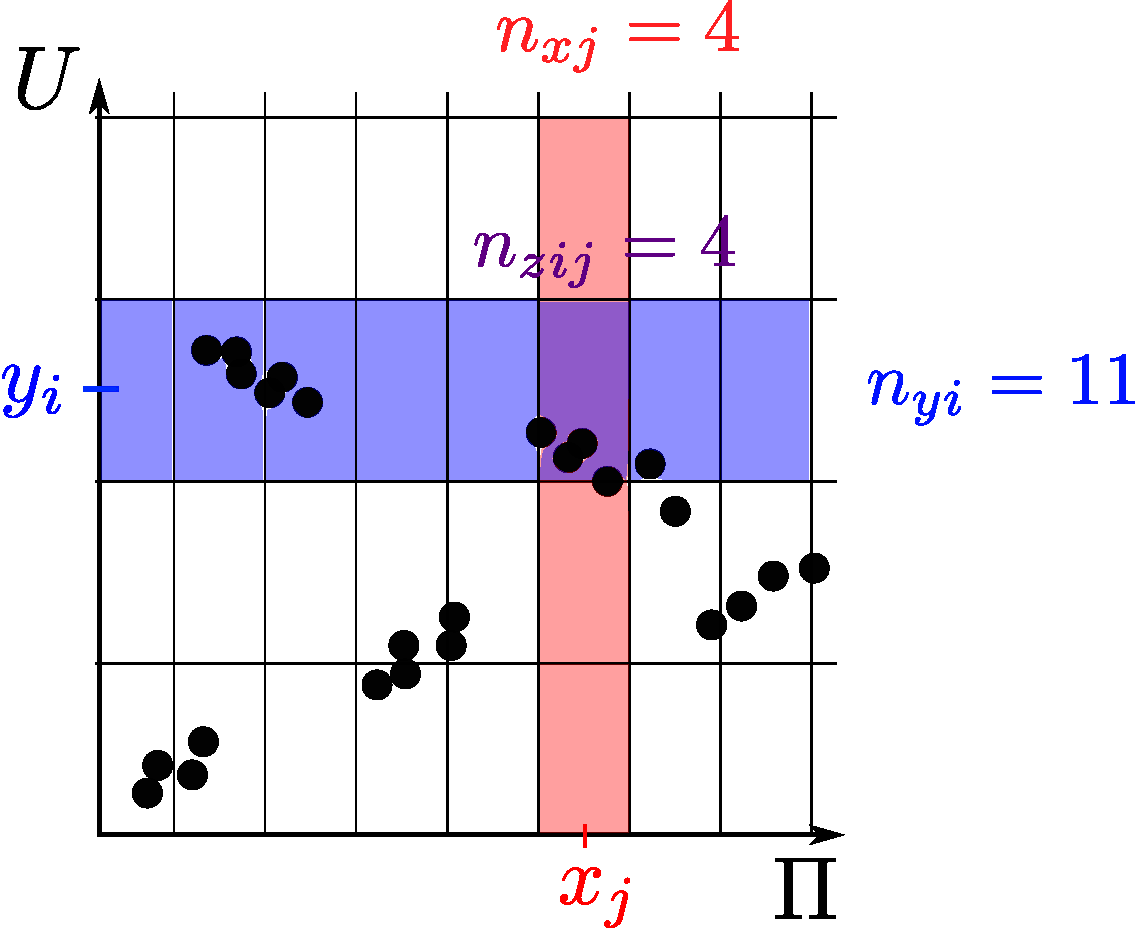
\includegraphics[width=\textwidth]{boxes}
    \caption{Méthode par histogrammes pour estimer les distributions des variables $U$ et $\bmu$. Les distributions sont estimées à partir de $n_{xj}$, $n_{yi}$ et $n_{zij}$, puis les valeurs de l'entropie $H$ et l'information mutuelle $I$ calculées.}
    \label{fig:binning}  
    \end{minipage}
    \hfill
    \begin{minipage}{0.4\textwidth}    
            \centering
            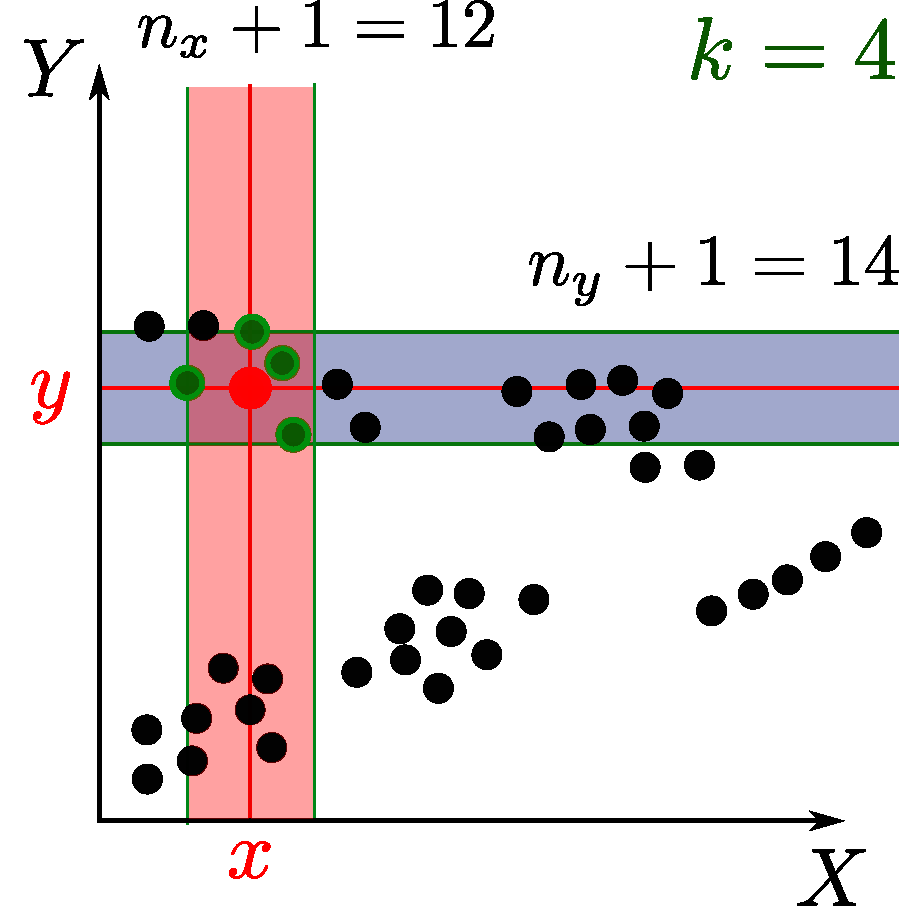
\includegraphics[width=0.8\textwidth]{kraskov.pdf}
            \caption{Découpage en KNN de Kraskov pour estimer l'entropie et l'information mutuelle des variables $X$ et $Y$. Les plus proches voisins du point rouge sont trouvés, en vert, et le processus est répété sur tous les points. Les valeurs de $n_x$ et $n_y$ permettent d'estimer directement l'entropie.}
            \label{fig:kraskov}
    \end{minipage}
    \end{figure}

\subsubsection{Choix de la méthode et des paramètres d'estimation}

L'information mutuelle mesure l'existence d'une relation statistique, linéaire ou non linéraire, entre les deux distributions. La figure~\ref{fig:exemple-limite} présente deux exemple de relations entre les variables $U$ et $\bmu$.
Dans le cas de gauche, la relation se rapproche d'une relation fonctionnelle, qu'on souhaite dans le cas de CxSOM, mais cette relation est bruitée. Dans le cas de droite, la relation n'est pas une fonction, mais elle est "précise": une valeur de $\bmu$ correspond à deux valeurs de $U$ et pas plus.
Nous avons calculé l'indicateur $I_x$ sur les deux distributions, estimé avec la méthode des histogrammes de Kraskov. La méthode de Kraskov est considérée comme donnant une valeur plus proche de la valeur théorique de l'information mutuelle que la méthode par histogrammes. 

Dans le cas de gauche, la méthode de Kraskov donne un coefficient d'incertitude assez faible. En effet, une valeur de $\bmu$ correspond à tout un intervalle de valeurs pour $U$. Sur le cas de droite, sa valeur est plus haute. En effet, une valeur de $\bmu$ correspond à deux valeurs de $U$, ce qui donne plus d'information que dans le premier cas de figure. Ce n'est pas ce qu'on veut mesurer dans CxSOM: le bruit est accepté, tant que la relation se rapproche d'une fonction.
La méthode des histogrammes permet d'ignorer ce bruit en prenant une taille de découpe plus grande pour $U$. Grâce à la méthode par histogrammes, l'indicateur normalisé possède une valeur forte, proche de 1 dans le cas de la droite, et plus faible dans le cas du cercle.

Dans le cas de CxSOM nous ne souhaitons ainsi pas une estimation précise de l'information mutuelle.
Le but de l'indicateur est de mesurer une relation de type fonction entre $U$ et $\bmu$.
Cette relation peut être bruitée et imprécise localement: on cherche à mesurer si une valeur de $\bmu$ correspond à \emph{un unique} intervalle de $U$, et non plusieurs comme dans le cas d'une carte simple, dans laquelle deux valeurs de $U$ sont codée par une position de BMU, voir figure~\ref{fig:upi_chap4}.
Nous utiliserons donc l'indicateur $I_x$ pour CxSOM en l'estimant par la méthode des histogrammes, avec un découpage large pour $U$. Cette façon d'estimer permettra de gommer la dispersion locale sur la valeur de $U$ pour mesurer uniquement la relation fonctionnelle existant entre $U$ et $\bmu$.

L'indicateur $I_x$ doit ainsi être considéré plutôt comme un indicateur s'inspirant du coefficient d'incertitude que comme une estimation précise de cette valeur. 
C'est cette estimation large qui nous permettra d'évaluer qu'une carte a dissocié les positions de ses BMUs en fonction de $U$ et non seulement de son entrée externe.
L'estimation du coefficient par la méthode de Kraskov donne quant à elle une valeur précise de la quantité statistique qu'est le coefficient d'incertitude entre $U$ et $\bmu$.
Nous pouvons considérer cette quantité comme un deuxième indicateur différent de $I_x$, que nous noterons $UC$, étant donné qu'il s'agit d'une valeur précise du coefficient d'incertitude. 
Nous appliquerons dans la section suivante ces deux indicateurs à l'étude de l'évolution de l'apprentissage au sein d'une architecture.

\begin{figure}
    \centering
    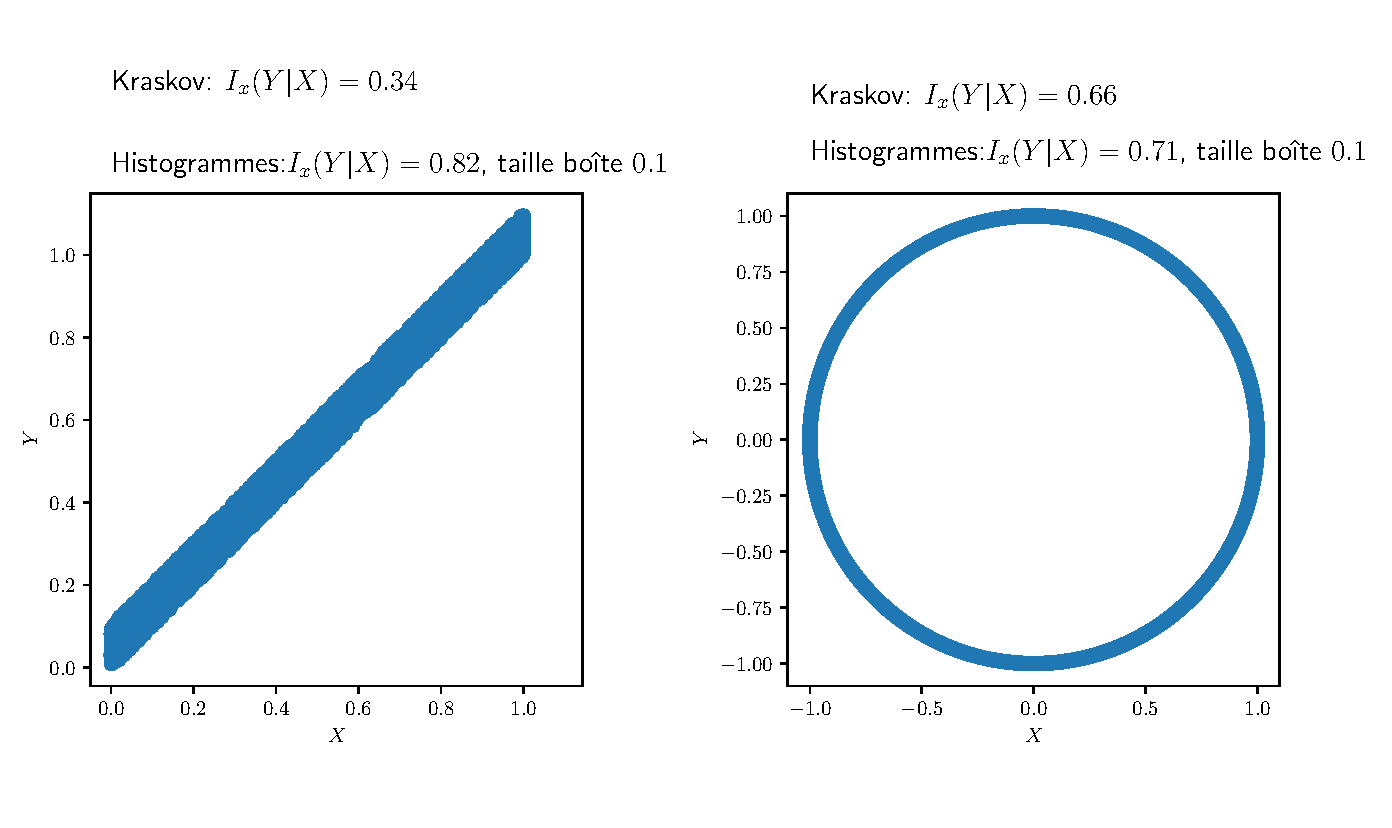
\includegraphics[width=0.75\textwidth]{comparaison_binning_kraskov.pdf}
    \caption{Comparaison du calcul de l'indicateur $I_x$ sur deux distributions. A gauche, la relation entre $Y$ et $X$ se rapproche d'une fonction, mais bruitée. A droite, la relation n'est pas fonctionnelle, mais de telle sorte qu'une valeur de $X$ correspond au maximum à deux valeurs de $Y$. Lorsqu'on calcule l'indicateur avec la méthode très granulaire de Kraskov, cet indicateur est plus élevé dans le cas de droite que de gauche: en effet, le calcul ne prend pas en compte si les points sont condensés ou éloignés. Pour que l'indicateur nous informe correctement sur l'aspect fonctionnel de la relation entre $X$ et $Y$, il faut enlever manuellement le bruit. Avec la méthode par histogrammes, on prend une taille de boîte de $0.1$ selon $Y$. Dans ce cas, l'indicateur est bien plus élevé à gauche, ou $Y$ se rapproche d'une fonction de $X$, que à droite.}
    \label{fig:exemple-limite}
    \end{figure}


\subsection{Application de l'indicateur $I_x$ au cas d'exemple multimodal simple}

Nous avons défini deux indicateurs à partir du coefficient d'incertitude. Premièrement, $I_x$, coefficient estimé par histogrammes avec de larges intervalles dans le découpage de $U$, permettant d'évaluer si $U$ est une fonction de $\bmu$, et autorisant une variation locale de $U$ pour une position de BMU.
En second lieu, $UC$, le coefficient d'incertitude estimée de façon précise avec une méthode d'estimation telle que les KNN de Kraskov.
Dans les deux cas, les indicateurs $I_x(U|\bmu)$ et $UC(U|\bmu)$ valent 1 lorsque $U$ est une fonction parfaite de $\bmu$. Cependant, $I_x$ nous permet de ne pas prendre en compte la dispersion des données au niveau d'une valeur de $U$ et permet d'évaluer si les BMUs sont différenciés selon $U$ dans une carte. 
$UC$ nous renseigne sur la valeur théorique du coefficient d'incertitude.

Le fait d'utiliser un indicateur numérique permet de tracer l'évolution de cet indicateur au cours de l'apprentissage des cartes.
Nous traçons cette évolution au cours de l'apprentissage dans un système de deux cartes apprenant sur le cercle en deux dimensions, l'exemple présenté au chapitre précédent.
Nous chercherons à vérifier que $I_x$ reflète bien la qualité de l'apprentissage dans une carte, puis nous utiliserons $UC$ pour évaluer l'information réellement portée par les cartes.

\subsubsection{Méthode expérimentale}

Pour cette expérience, une phase de test sur 5000 entrées est réalisée à intervalles réguliers lors de l'apprentissage, en utilisant le même jeu d'entrées pour chaque test. Chaque phase de test donne alors un ensemble d'entrées $\inpx\m{1}, \inpx\m{2}, U$ et un ensemble de réponses des cartes $\bmu\m{1}, \bmu\m{2}$. On peut alors estimer $I_x(U|\bmu\m{1})$ et $I_x(U|\bmu\m{2})$ sur chaque itération considérée et tracer la courbe de l'évolution de l'indicateur au long de l'apprentissage. 
Ces calculs sont réalisés sur 100 apprentissages séparé, prenant des entrées d'apprentissage aléatoires sur le même cercle. Les cartes sont initialisées à des poids aléatoires différents au début de chaque apprentissage. 
Les tracés représentent la moyenne, à chaque pas de temps, des indicateurs considérés au pas de temps $t$.

\subsubsection{Evolution de l'indicateur $I_x$ au cours de l'apprentissage}

Nous étudions d'abord l'évolution de $I_x$, calculé en discrétisant l'espace par la méthode des histogrammes.
On choisit de découper les valeurs de $U$ en 50 boîtes, et en 500 pour $\bmu\m{i}$: comme soulevé en section précédente, il est nécessaire d'utiliser un intervalle plus large pour les valeurs de $U$, afin de ne pas prendre en compte la dispersion des points au niveau local. Le tracé obtenu est tracé en figure~\ref{fig:MI_evol}.

Nous comparons les valeurs obtenues pour une carte de CxSOM à celles d'une carte simple apprenant sur les mêmes entrées $\inpx\m{1}$ ou $\inpx\m{2}$.
On s'attend à ce que l'information soit plus élevée pour la carte au sein de CxSOM que la carte seule. Cela montrera qu'une carte porte de l'information sur son entrée externe mais également sur le modèle global $U$, donc sur l'autre entrée.
On s'attend également à ce que cette valeur atteigne 1, ce qui montrerait qu'une seule carte porte de l'information sur tout le modèle: $U$ est une fonction de $\bmu$ dans chaque carte.

L'observation du tracé montre que les quantités $I_x(U|\bmu\m{1})$ et $I_x(U|\bmu\m{2})$ sont bien toutes deux plus élevées à chaque moment de l'apprentissage que dans le cas ou les cartes sont séparées; la valeur s'approche de 1 dans le cas de CxSOM.
Ces quantités augmentent au cours de l'apprentissage, traduisant bien un gain d'information des cartes sur le modèle au cours de l'apprentissage.

Nous pourrons donc utiliser $I_x$ comme indicateur d'une relation fonctionnelle entre $U$ et $\bmu$ dans chaque carte, en choisissant bien la taille de discrétisation pour $U$ lors de l'estimation. La taille de l'intervalle doit être assez élevée pour englober le bruit local des données, mais suffisamment faible pour détecter une séparation entre deux intervalles de $U$ codé par une même position de BMU.

\begin{figure}
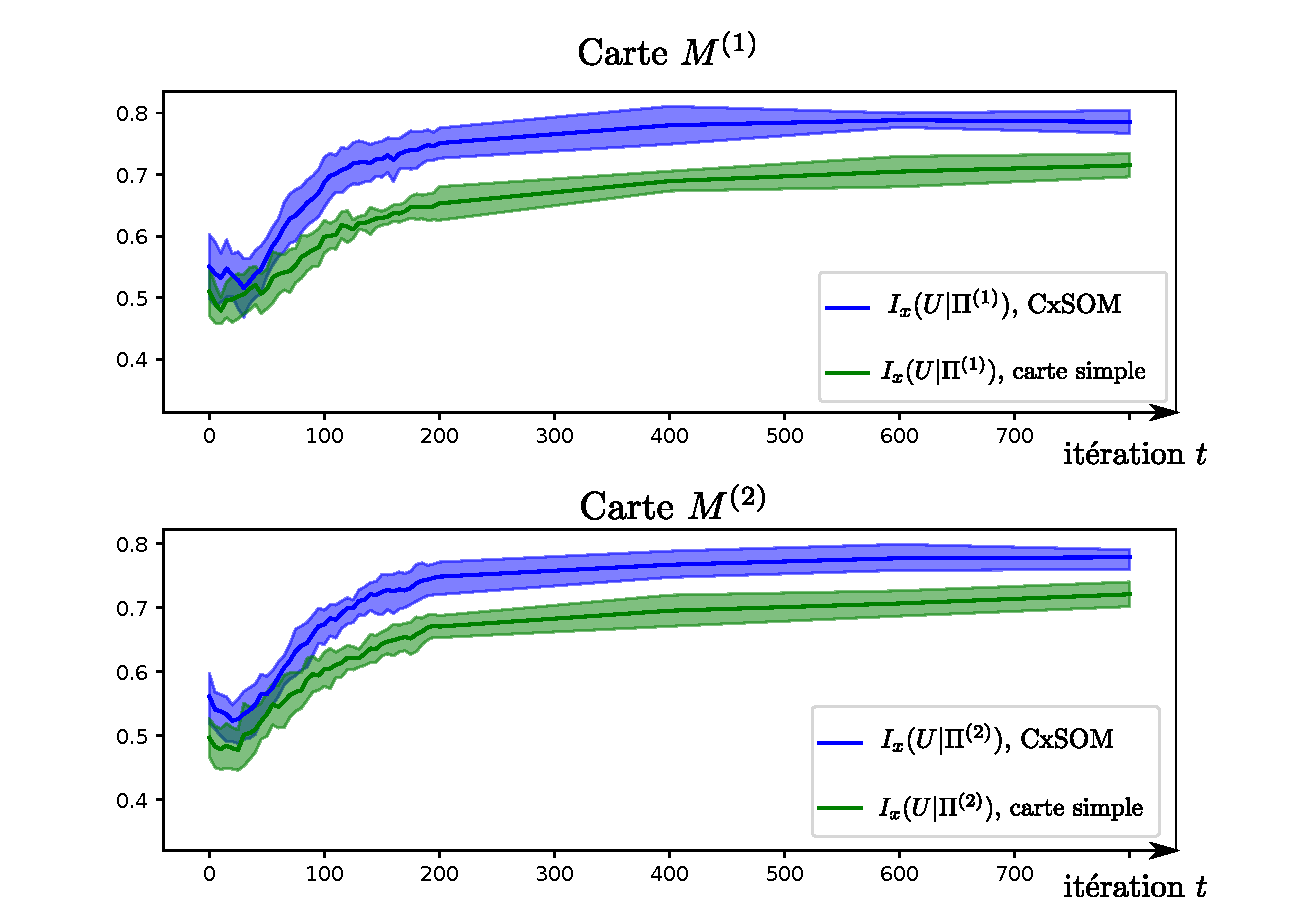
\includegraphics[width=\textwidth]{evolution_MI_binning}
\caption{Evolution de l'information mutuelle normalisée $I_x(U|\bmu)$ dans chaque carte au long de l'apprentissage. La courbe bleue correspond à $I_x(U|\bmu)$ dans l'architecture de cartes $M\m{1}$ et $M\m{2}$. On compare cette évolution à l'évolution de l'information d'une seule carte apprenant sur les mêmes entrées $X$ ou $Y$, sans être connectée.}
    \label{fig:MI_evol}
\end{figure}

\subsection{\'Evolution du coefficient d'incertitude théorique au cours de l'apprentissage}

Nous avons proposé $I_x$ comme indicateur pour évaluer la relation fonctionnelle entre $U$ et $\bmu$ et noté qu'il est nécessaire de l'estimer par histogrammes pour l'interpréter de cette façon dans le cadre de CxSOM.
Nous sortons de l'étape de validation de l'indicateur $I_x$ cherchant à évaluer une relation fonctionnelle autorisant le bruit local, pour étudier l'évolution du coefficient d'incertitude $UC$ entre les distributions de $U$ et de $\bmu$, estimée cette fois de façon précise, avec la méthode de Kraskov.
Le but est de comparer l'évolution du coefficient d'incertitude dans une carte CxSOM avec l'évolution dans une carte simple. Cet indicateur représente maintenant vraiment le taux l'information portée par une valeur $\bmu$ sur une valeur de $U$.

En figure~\ref{fig:MI_evol_total}, nous tracons l'évolution de $UC$.
Sur les tracés, il converge vers une valeur similaire à la fin de l'apprentissage pour la carte simple que pour la carte au sein d'une architecture CxSOM (tracés rouges et noirs). La valeur de $UC$ pour une carte dans CxSOM est même plutot inférieure à la valeur prise dans une carte simple.
Ce résultat est étonnant: cela signifie donc que la carte au sein de CxSOM n'a pas plus d'information sur le modèle qu'une carte isolée. Ce résultat va également à l'encontre de ce qu'on observe sur l'évolution de l'information mutuelle calculée par les histogrammes, dans laquelle une différence franche est observée entre la carte isolée et la carte au sein de l'architecture.

Proposons une explication.
On observe que l'information $UC(U|\bmu)$ tend vers une même valeur dans CxSOM et dans une carte isolée quand on la calcule avec l'estimateur de Kraskov, qui est proche de la valeur théorique de l'indicateur. Cela signifie qu'on a effectivement la même quantité d'information sur $U$ avec le BMU dans la carte isolée que dans CxSOM. Simplement, cette information n'est pas répartie de la même façon dans les deux expériences.
Dans une carte isolée, le niveau de quantification vectorielle qu'on effectue sur $\inpx$ est très précis: lorsqu'on présente une entrée $\inpx$ à la carte, le poids du BMU sera très proche de cette valeur $\inpx$. Or, la connaissance de $\inpx$ donne déjà beaucoup d'information sur le modèle $U$.
Dans CxSOM, on perd ce niveau de quantification sur $\inpx$, ce qu'on a observé en figure~\ref{fig:erreur}. On perd donc de l'information sur $\inpx$. 
Le fait que l'information mutuelle normalisée prenne la même valeur dans les deux expériences traduit alors qu'on a perdu de l'information sur l'entrée $\inpx$ par rapport à la carte isolée, avec la perte de précision, mais qu'on a en même temps gagné de l'information sur le modèle d'entrée, par la séparation selon $U$. Le fait que les deux évolutions de $I_x$, pour chaque expérience, convergent vers la même valeur montre qu'on est dans une situation de compromis: on gagne de l'information sur le modèle $U$, au détriment de l'information apprise sur l'entrée externe.
Ce comportement sera à valider sur d'autres modèles d'entrées.

C'est donc le fait de discrétiser grossièrement la distribution de $U$ qui permet de mesurer le gain d'information sur le modèle complet, sans prendre en compte le fait que la précision sur l'entrée externe est affaiblie. 
La comparaison de la valeur précise du coefficient d'intertitude, estimé par Kraskov, entre la carte simple et la carte dans CxSOM nous indique que la quantité d'information totale gagnée par une carte reste similaire dans le cas d'une carte simple qu'une carte dans CxSOM; elle est simplement répartie différemment entre les deux expériences.

\begin{figure}
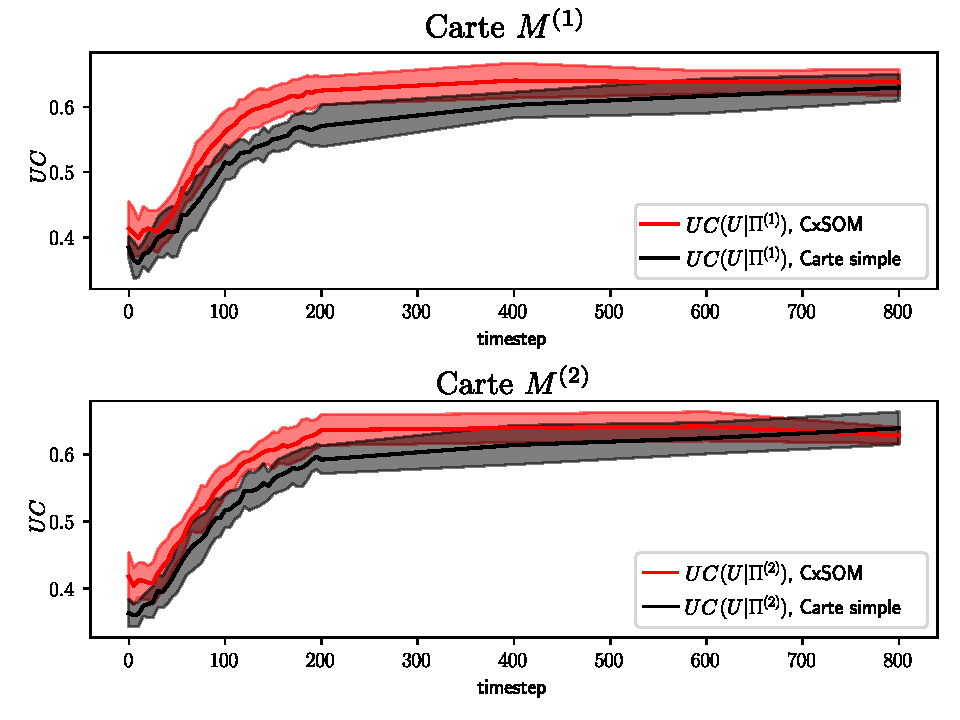
\includegraphics[width=\textwidth]{evolution_MI_K}
\caption{Evolution de $UC(U|\bmu)$ dans chaque carte au long de l'apprentissage, estimé par la méthode de Kraskov.\label{fig:MI_evol_total}}

\end{figure}

\section{Que nous apprend l'information mutuelle sur les données apprises par une carte de l'architecture ?}



\section{Conclusion}

Dans ce chapitre, nous avons introduit l'indicateur $I_x(U|\bmu)$, permettant de mesurer s'il existe une relation fonctionnelle entre $U$ et la position du BMU d'une carte. Cet indicateur s'appuie sur la notion de coefficient d'incertitude, une variante normalisée de l'information mutuelle. Le coefficient d'incertitude est une valeur probabiliste. L'indicteur $I_x$ que nous proposons correspond à l'estimation du coefficient d'incertitude par la méthide des histogrammes, en discrétisant l'espace des variables $U$ et $\bmu$, avec une grande taille d'intervalle pour $U$. Ce découpage permet de ne pas prendre en compte le fait que les valeurs de $U$ encodées par une position de BMU $\bmu$ ont une dispersion locale, un bruit. Dans ce cas, l'indicateur permet d'évaluer numériquement si un BMU code pour un seul intervalle de valeur pour $U$ et non plusieurs comme dans le cas d'une carte simple.
Cet indicateur permet de comparer les expériences entre elles, donnant une valeur normalisée entre 0 et 1.
Il est cependant limité par la dimension des variables $U$ et $\bmu$: l'estimation par histogrammes, nécessaire, nécessite trop de points en dimension supérieure à 2 ou 3.
L'information mutuelle et l'entropie étant des quantités fondamentales en théorie de l'information, il existe de nombreuses méthodes d'estimations de ces valeurs malgré la difficulté qu'elle pose, voir~\cite{Doquire2012ACO} pour une revue de différentes méthodes. 
Ainsi, l'utilisation de l'information mutuelle normalisée comme indicateur restera possible pour des données de plus grande dimension ou pour plus de cartes, mais son estimation devra être réétudiée pour s'adapter à ce type de données, en prenant en compte la gestion de la dispersion locale de $U$.


Parallèlement à la définition de cet indicateur, nous avons étudié l'évolution de la valeur exacte du coefficient d'incertitude lors de l'apprentissage d'une architecture de deux cartes de Kohonen. Cette valeur nous montre que CxSOM réalise un compromis lors de l'apprentissage de données: une carte de l'architecture perd de l'information sur son entrée externe par rapport à une carte simple apprenant sur les mêmes entrées, pour gagner de l'information sur le modèle global d'entrées. Finalement, la quantité d'information sur $U$ reste similaire dans le cas d'une carte simple ou d'une carte dans CxSOM, mais se répartit différemment.
Cette propriété reste à généraliser pour des distributions d'entrée différentes, comme les autres propriétés des cartes de CxSOM entrevues dans le chapitre précédent. La généralisation de toutes ces propriétés fera l'objet du chapitre suivant.
Elle pose néanmoins une question concernant la création d'architectures contenant plus de cartes: jusqu'à quel point une carte peut-elle se permettre de perdre de l'information sur l'entrée externe pour gagner de l'information sur le modèle ? 

\ifSubfilesClassLoaded{
    \printbibliography
    %\externaldocument{../main.tex}   
}{}
\end{document}

